\chapter{Related works}
\label{cha:related} 

\section{Background of Link Rates Schemes}
\label{sec:intro}

IEEE 802.11 ......... (以下略)

(放一篇ref, Fig跟Table當例子)

Each data rate is associated with a certain $SINR$ threshold. The method of selecting an appropriate link rate for transmitting/retransmitting packets is generally comprehended as the link (rate) adaptation mechanism.

The most commonly used rate adaptation technique is perhaps auto-rate fallback (ARF), which is widely implemented in present wireless devices \cite{Kamerman-bell-97}.

%%%%%%%%%%%%%%%%%%%%%%%%%%%%%%%%%%%%%%%%%%%%%%%%%%%%%%%%%%%%%%%%%%%%%%%%%
\begin{figure}
\begin{center}
\centering{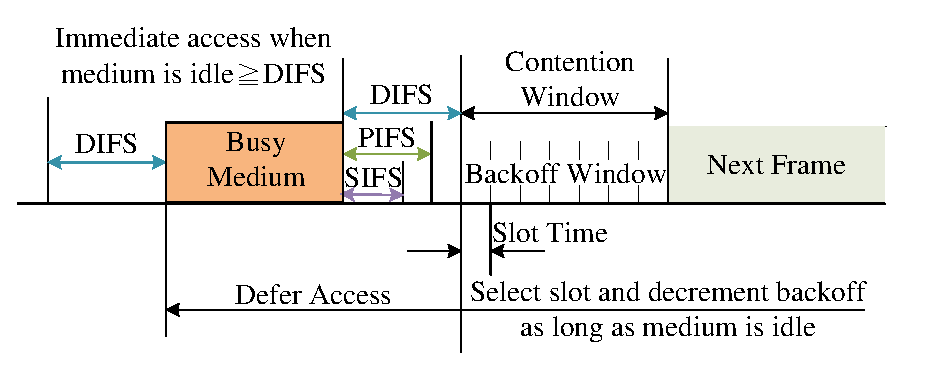
\includegraphics[width=9cm]{eps/DCF.eps}}
\caption{IEEE 802.11 MAC mechanism.}
\label{fig:DCF}
\vspace{-0.4cm}
\end{center}
\end{figure}
%%%%%%%%%%%%%%%%%%%%%%%%%%%%%%%%%%%%%%%%%%%%%%%%%%%%%%%%%%%%%%%%%%%%%%%%%


%%%%%%%%%%%%%%%%%%%%%%%%%%%%%%%%%%%%%%%%%%%%%%%%%%%%%%%%%%%%%%%%%%%%%%%%%
\begin{table}[!htb]
%\renewcommand{\arraystretch}{1.0}
\caption{$optCW$ estimation for IEEE 802.11b}
\begin{center}
\scalebox{0.65}
{\begin{tabular}{|c|c|c|c|c|c|c|c|c|}
%Row: 1
\hline
{$M$}
& {$p_{opt}^{r_{1}}$} & \small{$optCW^{r_{1}}$}
& {$p_{opt}^{r_{2}}$} & \small{$optCW^{r_{2}}$}
& {$p_{opt}^{r_{3}}$} & \small{$optCW^{r_{3}}$}
& {$p_{opt}^{r_{4}}$} & \small{$optCW^{r_{4}}$} \\
%Row: 2
\hline\hline
{10} & {0.0112} & {177} &{0.0155}&{128}&{0.0243}&{81}&{0.0320}&{61} \\
%Row: 3
\hline
{15} & {0.0074} & {271}&{0.0102}&{196}&{0.0159}&{125}&{0.0210}&{94} \\
%Row: 4
\hline
{20} & {0.0055} & {364}&{0.0076}&{263}&{0.0119}&{168}&{0.0157}&{127} \\
%Row: 5
\hline
{25} & {0.0044} & {458} &{0.0060}&{331}&{0.0094}&{211}&{0.0125}&{159} \\
\hline
%Row: 6
{30} & {0.0036} & {551}&{0.0050}&{398}&{0.0078}&{254}&{0.0104}&{191} \\
\hline
%Row: 7
{35} & {0.0031} & {645}&{0.0043}&{466}&{0.0067}&{297}&{0.0089}&{224} \\
\hline
%Row: 8
{40} & {0.0027} & {738}&{0.0037}&{533}&{0.0059}&{340}&{0.0078}&{256} \\
\hline
\end{tabular}}
\vspace{-0.2cm}
\end{center}
\label{table:optCW}
\end{table}
%%%%%%%%%%%%%%%%%%%%%%%%%%%%%%%%%%%%%%%%%%%%%%%%%%%%%%%%%%%%%%%%%%%%%%%%%

%%%%%%%%%%%%%%%%%%%%%%%%%%%%%%%%%%%%
%\vspace{0.5cm}
\begin{algorithm}[!htb]
\small
\caption{EARC Algorithm at Receiver}
\algsetup{indent=1em}
\begin{algorithmic}[1]
\WHILE{(DATA packet transmitted at rate $r_{i}$ received)}
\STATE  Look up the RSR table and decide a best sustainable rate $r_{j}$ based on $E_{rx}$;
    \IF{($i$ != $j$)}
    \STATE {\bf EARC Rate Flag} set to {\it true};
    \STATE Set value($b_1$$b_2$$b_3$) = $j-1$ in the {\bf EARC Control} field;

    \ELSE
    \STATE {\bf EARC Rate Flag} set to {\it false};
    \STATE Compare $E_{rx}$ with $E_{tx}$ and calculate $E_{diff}$;
        \IF{($E_{diff}$ == 0)}
        \STATE {\bf EARC CW Flag} set to {\it false};

        \ELSE
        \STATE {\bf EARC CW Flag} set to {\it true};
            \IF{($E_{diff} < 0$)}
            \STATE Set $b_1$ = 0; // to decrease CW
            \ELSE
            \STATE Set $b_1$ = 1; // to increase CW
            \ENDIF

            \IF{(($\frac{k}{K} < |E_{diff}| \le \frac{k+1}{K}$) \&\& (0 $\le k < K-1$))}
            \STATE Set value($b_2$$b_3$) = $k$;
            \ELSE
            \STATE Set value($b_2$$b_3$) = $K-1$;
            \ENDIF
        \ENDIF
    \ENDIF
\STATE Return ACK packet back to transmitter;
\ENDWHILE
\end{algorithmic}\label{alg:EARC-rx}
\end{algorithm}
%%%%%%%%%%%%%%%%%%%%%%%%%%%%%%%%%%%%

